
\documentclass[tikz,border=7pt]{standalone}
\usepackage[utf8]{inputenc}
\usepackage[T1]{fontenc}
\usepackage{amsmath}
\usepackage{xcolor}
\usetikzlibrary{arrows.meta,calc,angles,quotes,patterns,positioning}
\definecolor{brand}{HTML}{1E3A8A}
\definecolor{brandtwo}{HTML}{2563EB}
\definecolor{accentred}{HTML}{EF4444}
\definecolor{accentgreen}{HTML}{16A34A}
\definecolor{accentorange}{HTML}{F59E0B}
\definecolor{muted}{HTML}{64748B}
\definecolor{lightblue}{HTML}{EEF6FF}
\tikzset{force/.style={-{Latex[length=3mm]}, line width=1.15pt}, axis/.style={-{Latex[length=2mm]}, line width=.8pt, color=muted}, body/.style={draw=brandtwo, fill=lightblue, line width=1pt, rounded corners=2pt}, lab/.style={font=\small, text=brand}, sml/.style={font=\scriptsize, text=muted}}
\begin{document}

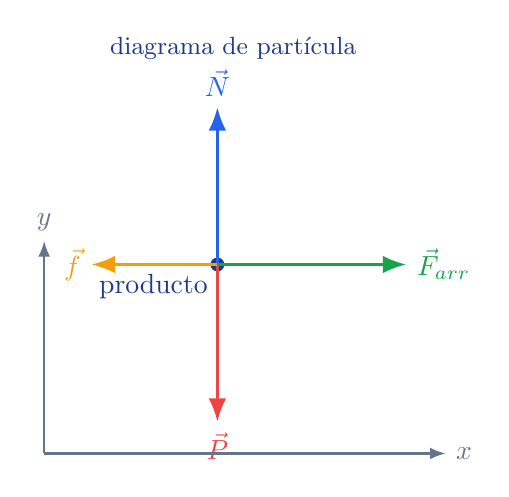
\begin{tikzpicture}[scale=1]
\fill[brand] (0,0) circle (2.5pt) node[below left] {producto};
\draw[force,color=brandtwo] (0,0)--(0,2) node[above] {$\vec N$};
\draw[force,color=accentred] (0,0)--(0,-2) node[below] {$\vec P$};
\draw[force,color=accentgreen] (0,0)--(2.4,0) node[right] {$\vec F_{arr}$};
\draw[force,color=accentorange] (0,0)--(-1.6,0) node[left] {$\vec f$};
\draw[axis] (-2.2,-2.4)--(2.9,-2.4) node[right] {$x$}; \draw[axis] (-2.2,-2.4)--(-2.2,.3) node[above] {$y$};
\node[lab, align=center] at (.2,2.75) {diagrama de partícula};
\end{tikzpicture}

\end{document}